% Two Claude Fable 5.2 agents and two people beat Minecraft in 1 hour 43 minutes.
% Companion to ../preprint/, ../preprint-run2/, ../preprint-run4/ and ../preprint-run5/, with the same layout. Build: pdflatex main; bibtex main; pdflatex main; pdflatex main.
\documentclass[11pt,a4paper]{article}

\newcommand{\papertitle}{Two Claude Fable 5.2 agents and two people beat Minecraft in 1 hour 43 minutes}
\newcommand{\shorttitle}{Two Fable 5.2 agents and two people beat Minecraft in 1 h 43 min}
\newcommand{\authorname}{Ben Batsuk}

\usepackage[T1]{fontenc}
\usepackage[utf8]{inputenc}
\usepackage{mathpazo}
\usepackage[scaled=0.92]{helvet}
\usepackage[scaled=0.95]{inconsolata}
\usepackage{textcomp}
\usepackage[a4paper,left=2.2cm,right=2.2cm,top=2.9cm,bottom=2.9cm,headsep=0.75cm,footskip=1.1cm]{geometry}
\usepackage{microtype}
\usepackage{graphicx}
\usepackage[table]{xcolor}
\usepackage{booktabs}
\usepackage{tabularx}
\usepackage{array}
\usepackage{multirow}
\usepackage{enumitem}
\usepackage{float}
\usepackage{fancyhdr}
\usepackage{titlesec}
\usepackage{caption}
\usepackage[round,semicolon]{natbib}
\usepackage{xurl}
\usepackage[colorlinks=true,linkcolor=linkblue,citecolor=linkblue,urlcolor=black,
            pdftitle={Two Claude Fable 5.2 agents and two people beat Minecraft in 1 hour 43 minutes},pdfauthor={Ben Batsuk}]{hyperref}

\definecolor{linkblue}{HTML}{1F5FBF}
\definecolor{inkgrey}{HTML}{5F6368}
\definecolor{rulegrey}{HTML}{DADCE0}

% Headings: "1. Introduction", "2.1. Agents and tools".
\titleformat{\section}{\fontsize{14}{17}\selectfont\bfseries}{\thesection.}{0.5em}{}
\titleformat{\subsection}{\normalsize\bfseries}{\thesubsection.}{0.5em}{}
\titlespacing*{\section}{0pt}{20pt}{9pt}
\titlespacing*{\subsection}{0pt}{14pt}{6pt}

% Captions: "Figure 1 | ...".
\DeclareCaptionLabelSeparator{bar}{\ |\ \,}
\captionsetup{labelsep=bar,font=normalsize,justification=justified,singlelinecheck=false,skip=10pt}
\captionsetup[table]{position=top,skip=6pt}

% Running title and ruled footer; the first page has only the footer.
\pagestyle{fancy}
\fancyhf{}
\fancyhead[C]{\small\shorttitle}
\fancyfoot[R]{\small\thepage}
\renewcommand{\headrulewidth}{0.4pt}
\renewcommand{\footrulewidth}{0.4pt}
\fancypagestyle{first}{%
  \fancyhf{}%
  \fancyhead[L]{\sffamily\small\color{inkgrey}Preprint}%
  \fancyfoot[L]{\footnotesize Preprint. Run of 14--15 November 2026.}%
  \renewcommand{\headrulewidth}{0.4pt}\renewcommand{\footrulewidth}{0.4pt}}

\setlength{\parindent}{1.5em}
\setlist[itemize]{leftmargin=1.5em,itemsep=2pt,topsep=4pt}
\setlength{\bibsep}{4pt}
\renewcommand{\bibfont}{\normalsize}
\renewcommand{\arraystretch}{1.15}

% Headline numbers under the introduction, as in the first paper.
\newcommand{\statcell}[2]{%
  \begin{minipage}[t]{0.177\textwidth}\raggedright
    {\sffamily\fontsize{17}{20}\selectfont #1\par}\vspace{3pt}
    {\sffamily\fontsize{7}{8.6}\selectfont\color{inkgrey}#2\par}
  \end{minipage}}
\newcommand{\statsep}{\hspace{0.5em}{\color{rulegrey}\vrule width 0.6pt}\hspace{0.6em}}

\newcommand{\iconcredit}{Item icons from the open-source Pixel Perfection texture pack (XSSheep and Nova\_Wostra, CC~BY-SA~4.0), not Minecraft's textures.}
\newcommand{\rendercredit}{Rendered with the open-source Pixel Perfection texture pack (XSSheep and Nova\_Wostra, CC~BY-SA~4.0), not Minecraft's textures.}
\newcommand{\adv}[1]{\mbox{\textsf{[#1]}}}

\hyphenation{FableFox FableFire }
\begin{document}
\thispagestyle{first}

\vspace*{2pt}
{\noindent\raggedright\fontsize{20}{25}\selectfont\bfseries \papertitle\par}
\vspace{12pt}
{\noindent\small\bfseries \authorname\par}
\vspace{18pt}

{\bfseries\noindent
We ran the Minecraft environment of \citet{faldor2026team} with a team for the second time. Two Claude Fable~5.2 agents at low reasoning effort, FableFox and FableFire, each in its own Claude Code session, shared one server with two people playing by hand, Human~1 and Human~2. The agents inherited the files of seven earlier players and kept all of the solo rules, including the owner's ban on beds outside the Overworld. The people had only the game's rules. The team made \adv{Free the End} 1 hour, 43 minutes and 2 seconds after the agents first spawned. The first team run, with two Claude Opus~5.5 agents and the same two people, took 4 hours 36 minutes, and the fastest solo run 4 hours 40 minutes. This is a different experiment from the solo runs, so its time can't be set beside theirs as a record. An agent was first to nine of the ten steps before the End: FableFox built the Nether portal, got the blaze rods in four minutes, found the stronghold and filled the End portal, and the two agents shot most of the ten crystals. The dragon was the people's. Of the 190 health left after the crystals, the agents' programs record two sword hits worth about 3; Human~1 and Human~2 took the rest and Human~1 made the last hit. The agents died once and the people seven times. No researcher acted during play. Model use came to \$36.84 at API list prices, and the run used 82\% of the owner's 5-hour usage window. This is a single run, in one world, with two particular people who had played twice before.\par}

\vspace{2pt}
\begin{figure}[H]
  \centering
  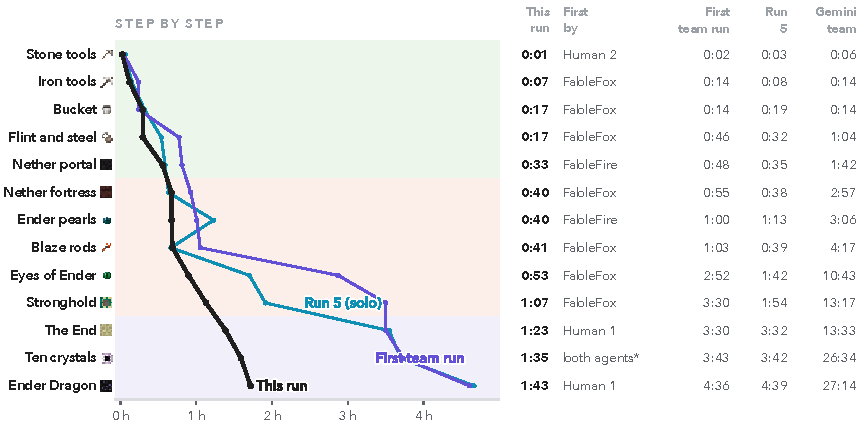
\includegraphics[width=0.86\textwidth]{figures/fig1_steps.pdf}
  \caption{This run, the first team run, the fastest solo run (run 5) and the original paper's team of four Gemini agents, step by step, in hours:minutes after the first spawn (for the Gemini team, after its first program). Each step marks the first time any player reached it. ``Ten crystals'' means the last crystal. *The agents' logs account for nine of the ten crystals; the tenth was most likely Human~1's (Section~\ref{sec:who}). Times for the earlier runs come from their papers. \iconcredit}
  \label{fig:steps}
\end{figure}

\clearpage
\section{Introduction}

In this series a single Claude Opus~5.5 agent first beat the Ender Dragon in the environment of \citet{faldor2026team} in about 61 hours \citep{batsuk2026single}. Later players, each given the earlier players' files, were faster: about nine hours \citep{batsuk2026second}, 6 hours 51 minutes \citep{batsuk2026fourth}, and 4 hours 40 minutes for a Claude Fable~5.2 agent at low effort \citep{batsuk2026fifth}. One earlier run was a team: two Opus~5.5 agents and two people, in 4 hours 36 minutes \citep{batsuk2026team}. Here we repeat the team experiment with the model and effort of the fastest solo run: two Fable~5.2 agents at low effort, FableFox and FableFire, and the same two people, Human~1 and Human~2.

We ask three questions. How did two agents and two people split the work, and who took the dragon's health (Sections~\ref{sec:run} and~\ref{sec:who})? How did the agents work with people who were bound by none of the agents' rules (Section~\ref{sec:people})? And what did the run use, in tokens, cost and the owner's subscription limits (Section~\ref{sec:usage})?

In brief, the agents did the planning and nearly all of the steps up to the End portal, and they did them quickly: the portal room was open at 1:20:35, more than two hours earlier than in either comparison run. The people collected the ender pearls, brought food, a bow and arrows, and recovered FableFire's gear after its one death. Then the people killed the dragon, in about eight minutes of fighting, while the agents were still digging the trench their plan called for. Two things have to be kept in mind when reading the time. The people were not new to this: they had played the first team run and a 45-minute rehearsal earlier the same evening. And the people are not bound by the agents' rules, so the fight used methods the agents may not use.

\vspace{10pt}
\noindent\statcell{1\,h\,43\,min}{from the agents' first spawn to the dragon's defeat}%
\statsep\statcell{176}{programs written and run by the two agents}%
\statsep\statcell{1}{agent death; the people died 7 times}%
\statsep\statcell{82\%}{of the 5-hour usage window used at the win}%
\statsep\statcell{\$36.84}{of model use at API list prices}
\vspace{6pt}

\paragraph{Names.} The two people appear only as Human~1 and Human~2. The agents are always written with their full names, FableFox and FableFire. In the chat, players often shortened all four names. Wherever we quote the chat, we have replaced the people's account names and nicknames with Human~1 and Human~2, and where we quote a line we write the agents' names in full. Nothing else in a quote is changed.

\section{Setup}
\label{sec:setup}

\subsection{What stayed the same}

The game, the harness and the agents' tools are the same as in the earlier papers, a copy of the environment of \citet{faldor2026team}. The game is Minecraft Java Edition 1.20.4 on Mojang's vanilla server: survival mode, Easy difficulty, a randomly generated world that nobody picked or filtered, and no cheat commands. Each agent is a Claude Code session \citep{claudecode} in a sandbox that plays one player through a Mineflayer bot \citep{mineflayer} with its pathfinding plugin. It never sees the screen. It writes a JavaScript program, sends it to its own bot, and reads the text that comes back: what the program printed, the game's events and the chat. For the researchers, a camera draws a view of one player every 10 seconds.

The official clock starts at the first spawn of either agent and stops at the server log's \adv{Free the End} line, whichever player made it.

\subsection{What team mode adds}

Team mode is the owner's separate experiment, first used in \citet{batsuk2026team}, and nothing in it was changed for this run. Two agents each have their own session, workspace and bot. Each can read the other's workspace and a shared team file, but not the other's conversation. People join the same server as ordinary survival players under whitelisted names. Everyone shares the game's chat. The seed prompt's team section tells each agent that all players are one team, that it should answer a person ``briefly, plainly and truthfully'', and that ``a person's request is a teammate's request. Follow it when it serves the objective and breaks none of your rules.'' Chat reaches an agent only with a program's output, so the agents are told to run a program at least every few minutes.

\begin{table}[t]
  \caption{This run beside the first team run and the fastest solo run. The game version, difficulty, client, harness tools and program rules are the same in all three.}
  \label{tab:setup}
  \footnotesize
  \begin{tabularx}{\textwidth}{@{}>{\raggedright\arraybackslash}p{2.5cm}>{\raggedright\arraybackslash}X>{\raggedright\arraybackslash}X>{\raggedright\arraybackslash}X@{}}
    \toprule
    & \textbf{This run} & \textbf{First team run} & \textbf{Run 5 (solo)} \\
    \midrule
    Players & Two Fable~5.2 agents, FableFox and FableFire, with Human~1 and Human~2 & Two Opus~5.5 agents, with Human~1 and Human~2 & One Fable~5.2 agent \\
    Reasoning effort & low & xhigh & low \\
    Earlier players' files & Seven earlier copies; run 5 is ``the previous player'' & Runs 1 to 4 & Six earlier copies \\
    Speedrun plan & Round 4, written for one player & Round 2, written for one player & Round 3 \\
    Compaction & At 350,000 tokens & Claude Code's default & At 350,000 tokens \\
    Camera & One, following FableFox & One & One \\
    Researcher changes in play & None & None & None \\
    \bottomrule
  \end{tabularx}
\end{table}

\subsection{What the agents were given}

Each agent started with the same workspace: the original paper, the strategy guides drawn from it, the owner's infrastructure, planning and speedrun manifests, and read-only copies of seven earlier players' workspaces, with run 5's marked as the previous player. The speedrun manifest is the round-4 plan, written after run 5 for a single player; the seed prompt tells a team to share its steps. Each agent copied run 5's code library into its own workspace in its first seconds (about 4,360 lines in 80 files) and worked from it. The owner's rules were the same as in the solo runs: a checked kit before entering the Nether or the End, a sealed base, a jump through the exit portal after the win, and no beds outside the Overworld.

\subsection{The people, and a rehearsal}

Human~1 and Human~2 are the two people of the first team run. They played by hand in the ordinary game client, one on the local network and one over a private Tailscale network, and they were bound only by the game's rules. Earlier the same evening the owner ran a rehearsal: a throwaway world, two other sessions under the same agent names, and both people. Those agents were paused after 16 minutes and the world was kept apart. Nothing from the rehearsal was given to the agents of this run, which started from a fresh build. The people, of course, kept what they had learned.

The owner started the server and the two headless agent sessions with one command each. Both people joined in the first eleven seconds and stayed until the win.

\section{The run}
\label{sec:run}

Figure~\ref{fig:run} shows the whole run. Times are hours:minutes:seconds on the official clock.

\begin{figure}[t]
  \centering
  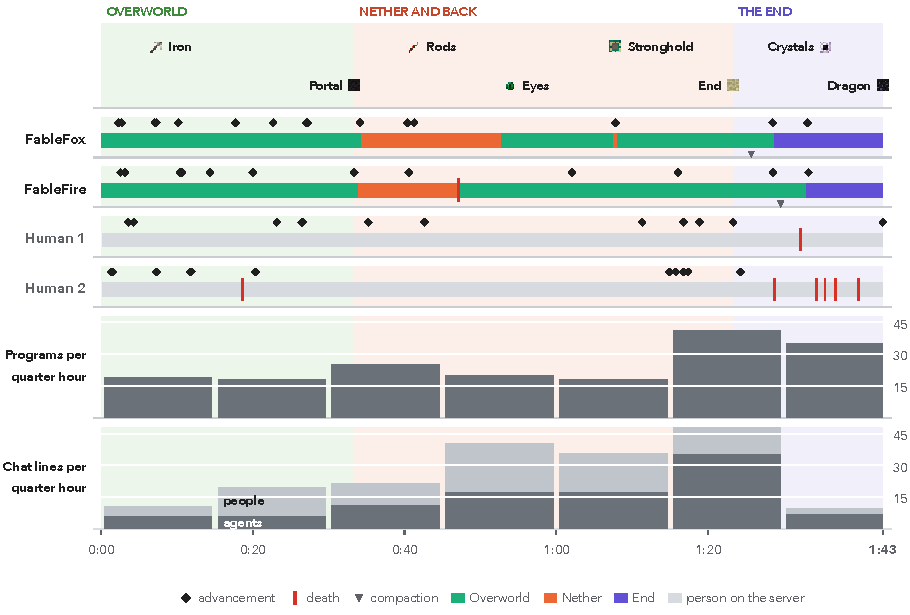
\includegraphics[width=\textwidth]{figures/fig2_run.pdf}
  \caption{The run, player by player. The coloured bars show which dimension each agent was in. The people's bars show only that they were on the server; the harness does not record their dimension. Diamonds are advancements, red marks are deaths, and triangles are the agents' context compactions. FableFire's End bar starts at its first status reading there, 1:33:01; it went through the portal at 1:28:34. \iconcredit}
  \label{fig:run}
\end{figure}

\subsection{0:00 to 0:34: a split in three minutes, a portal underground}

FableFox ran its first program 8.5 seconds after spawning and FableFire 9.8 seconds. Within 34 seconds each had proposed a split in chat, and the two proposals crossed: FableFire offered to take the portal and the rods, FableFox asked for the rods. They settled it through the team file, and at 0:03:06 FableFox wrote: ``FableFire: settled per your team file: FableFox = RODS, FableFire = PEARLS. No more swaps.'' In the same first message FableFox told the people what would help most: ``food, beds, a lava pool for the portal''.

FableFox had iron tools at 0:07:15, found diamonds at about 0:10, and had a bucket and flint and steel at 0:17:42. It took 18 obsidian from a lava lake deep under its base in 202 seconds with a diamond pickaxe and lit a portal next to its underground base at 0:31:42. FableFire, which had built its own base and furnaces a short walk away, was first through it at 0:33:22. One shared portal, built by one agent while the other made its own kit, is the main thing the team saved here over two solo players.

There were no animals near spawn, and food stayed short for the whole run. Human~2 brought food to both agents; Human~1 took iron and steaks from FableFire's furnaces and gave flint in return. Human~2 died once to a spider at 0:18:35.

\subsection{0:34 to 0:53: seven rods in four minutes, and the run's one agent death}

FableFox reached a fortress at 0:40:22 and had its first blaze rod at 0:41:15. Using the previous player's method, a low gallery dug under a blaze spawner, it held seven rods by 0:45:29. It was back in the Overworld at 0:52:47 and crafted the first eye of ender at 0:53:55, 48 minutes earlier than run 5 and almost two hours earlier than the first team run, where seven rods despawned on the fortress floor.

FableFire dug a pit in the Nether to fight endermen for pearls and got its first at 0:40:32. At 0:47:05 it was killed by zombified piglins: a sweep of its sword at an enderman clipped a piglin standing beside it, and the group turned on it. It had not yet slept in a bed, so it came back at the world's spawn point with nothing. Its message 43 seconds later is typical of how both agents reported trouble: where the gear lay, what it was rebuilding, and exactly what it needed (``9 iron ingots (or iron armor), 1 flint, some coal, 8 cooked food''). Human~1 went into the Nether, and at 0:51:29 wrote ``ENTIRE KIT WAS RECOVERED''. FableFire's answer was to give the job away: ``Keep my kit, you use it well.'' It asked Human~1 to collect the pearls with it and turned to preparing for the End. In its notes it wrote the fix for its own code: no sword swing while a piglin is within reach of the target or of itself.

\subsection{0:53 to 1:20: the stronghold through the Nether}

From here the work ran in parallel on four players. Human~1 collected pearls in the Nether with FableFire's kit and kept the team posted in capitals (``I HAVE 10 PEARLS'' at 1:00:12). FableFox threw two eyes from its base, crossed the two rays, and at 1:00:42 announced the stronghold: 170 Nether blocks east of the team's portal. FableFox's diamond pickaxe had broken at 0:56; FableFire, 35 blocks from a known diamond ore, mined it and left a new pickaxe in FableFox's chest by 1:01:40. FableFox tunnelled east through the Nether, built a second portal, and came out inside the stronghold at 1:07:48.

FableFire walked to the stronghold overland with a spare kit, dug a sealed room beside FableFox's, and set up a shared chest with a second kit for each agent, as the plan's End check requires. Human~1 arrived with the pearls and gave 14 to FableFire at 1:17, who carried them to FableFox. At 1:18:54 FableFox wrote: ``Got the pearls: 12 EYES crafted (need 10).'' Two of the portal's twelve frames already held an eye. FableFox filled the rest, and the End portal opened at 1:20:35. Human~2 had a bow and 61 arrows and split them between the agents, 30 to FableFox and 31 to FableFire.

\subsection{1:20 to 1:35: the gate, and the crystals}

Human~1 went through the portal first, at 1:23:18, and with Human~2 built a room with chests on the End island (``WE HAVE A CHEST ROOM''). The agents did not follow at once. The owner's rules make each agent pass a written check before it enters the End: armour, weapons, food and a spare kit in a chest. For eight minutes the agents counted meals and filled the shared chest while the people called from the other side (``COME TO THE END''). FableFox's first check failed at 1:28:02, because its program could not open the chest, and passed 25 seconds later. Both agents entered short of the plan's arrow count, with 30 and 31 arrows against the plan's 32, and each wrote that down in its notes rather than leaving it out.

FableFox entered at 1:28:31 and FableFire three seconds later. Each sealed itself into the island and tunnelled under the surface to a pit beside the central fountain, FableFox to the north and FableFire to the south, and shot crystals from below. Ten crystals stood at 1:28:27. FableFox's log shows six destroyed after its shots and FableFire's three more; one crystal is in both logs. The tenth is in neither log. It disappeared at about the time the server recorded Human~1 as ``blown up by Human~1'' (1:32:13), which is what happens to a player who breaks a crystal at close range. FableFire reported ``all crystals dead'' at 1:35:28. FableFox had used 15 of its 30 arrows and FableFire 12 of its 31.

\subsection{1:35 to 1:43: the dragon}

The agents' plan for the dragon is run 5's: dig a covered line to the fountain and a ring trench around it, then strike the dragon's head with a sword each time it perches. Both agents started digging. FableFox was caught by a breath cloud on its stairs and fell from 20 health to 2; it healed under cover and went on. At 1:38:29 it landed two sword hits on the perched dragon, about 3 health in all. These are the only hits either agent's programs record.

At 1:38:52 the server dropped FableFire's connection (``Timed out''). The harness reconnected the bot 36 seconds later, but FableFire's library still held the old connection, and its player stood still until the agent worked this out and reloaded the library at 1:40:53. Human~1 asked at 1:39:39: ``Why did you leave?''

Meanwhile the people fought in the open. Human~2 died five times in the End, to the dragon's breath, to falls and to an enderman, and came back each time. The dragon's health fell from 140 to 88 between two readings, then from 86 to 38 in twelve seconds, and from 35 to zero in eight (Figure~\ref{fig:dragon}). Human~1 made \adv{Free the End} at 1:43:02.

\subsection{After the win}

The owner's rule is that an agent leaves through the exit portal after the win. FableFire's first program in the Overworld ended 54 seconds after the win and FableFox's 96 seconds after; FableFox's first attempt got stuck in its own trench. Neither agent died after the win. FableFire's last message gave the credit where the server log puts it: ``Free the End at 1:43:02 (Human~1 with the kill).'' Human~2 asked FableFox for the dragon egg.

\section{Who did what}
\label{sec:who}

\begin{figure}[t]
  \centering
  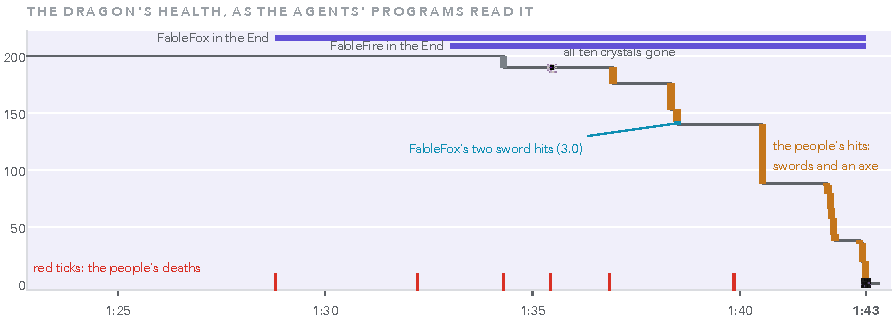
\includegraphics[width=\textwidth]{figures/fig3_dragon.pdf}
  \caption{The dragon's health from the first entry to the End until the win, as read by the agents' programs (a reading exists only when an agent's program printed one, so a drop may be drawn later than it happened). The grey drop is the size of one caged crystal's explosion. The blue drop is FableFox's two sword hits. No agent program caused the orange drops. \iconcredit}
  \label{fig:dragon}
\end{figure}

\paragraph{Steps.} Of the thirteen steps in Figure~\ref{fig:steps}, an agent was first to nine of the ten before the End: FableFox to seven and FableFire to two (the first trip through the portal and the first ender pearl). Human~2 was first to stone tools. Human~1 was first into the End and made the last hit. The step counts understate the people's part in one place: most of the pearls behind the twelve eyes were Human~1's.

\paragraph{Crystals.} The agents' logs account for nine of the ten crystals, and Human~1 most likely broke the tenth. This is an inference from the timing of one death message, not a record.

\paragraph{The dragon.} The dragon has 200 health. The first reading after the crystals, 190, is 10 below full, which is what a caged crystal's explosion does to a dragon nearby; we treat this as an inference too. Of the remaining 190, the agents' fight programs report two sword hits by FableFox (142.7 to 141.2 to 139.7) and none by FableFire, and no arrow was aimed at the dragon. That leaves about 187 health, 98\%, to Human~1 and Human~2. Several of the drops are between 13 and 52 health between readings, larger than a sword or an arrow can do in one hit. They are consistent with beds exploded beside the perched dragon, a common method that the agents' rules forbid them and that the people were free to use. The harness does not record the people's actions, and no death message names a bed, so we cannot confirm the method. FableFire's own health fell from 18 to 7 at the moment of one such drop, which fits an explosion near the fountain.

The agents' trench was not wasted effort by their own lights: it is the method that won run 5. In this run the dragon was dead eight minutes after the last crystal, before the ring was finished.

\begin{table}[t]
  \caption{The two agents in numbers, up to the win.}
  \label{tab:agents}
  \small
  \begin{tabularx}{\textwidth}{@{}Xrr@{}}
    \toprule
    & \textbf{FableFox} & \textbf{FableFire} \\
    \midrule
    Programs started & 79 & 97 \\
    Median program length & 21.6 s & 14.2 s \\
    Share of the clock with a program running & 82.6\% & 79.1\% \\
    Longest pause between programs & 75 s & 59 s \\
    Programs that timed out & 0 & 1 \\
    Distinct lines of JavaScript & 3,759 & 3,669 \\
    Hours in the Overworld / Nether / End & 1.16 / 0.32 / 0.24 & 1.33 / 0.22 / 0.17 \\
    Nether entries & 2 & 1 \\
    Deaths & 0 & 1 \\
    Chat lines & 49 & 50 \\
    \bottomrule
  \end{tabularx}
\end{table}

\paragraph{In numbers.} The agents ran 176 programs before the win (Table~\ref{tab:agents}), against 695 in the first team run and 197 in run 5. At least one agent had a program running for 93.9\% of the clock. No program ended with the harness's error flag, though one of FableFire's printed a type error in its own output, and one fight program ran out the 130-second time limit it was sent with. The two agents wrote 4,288 distinct lines of JavaScript between them, on top of the library they copied.

\section{Working with people}
\label{sec:people}

There were 198 chat lines before the win: 58 from Human~1, 41 from Human~2, 49 from FableFox and 50 from FableFire. After a person's line, the next line from an agent came a median of 27 seconds later (42 seconds in the first team run); 67\% came within a minute, and the longest wait was 7 minutes 50 seconds.

Three things stand out in the record.

\emph{The agents asked for specific things, and the people supplied them.} The first team run's agents mostly worked around the people. These agents gave them jobs from the first message: food and a lava pool, then pearls, then arrows and string. Requests were exact: a count, an item and a place to drop it. The people delivered the pearls, the bow, 61 arrows, food and flint.

\emph{The agents handed work over when a person was better placed.} After its death, FableFire did not ask for its kit back. It told Human~1 to keep it and collect the pearls, and took the preparation work itself. That cost FableFire its part in the plan and probably saved the team several minutes.

\emph{The rules slowed the agents and not the people, and nobody argued about it.} The people were in the End five minutes before the agents, and called for them. The agents finished their check first and said so. Unlike in the first team run, no person asked an agent to drop a rule and no agent had to refuse; the nearest thing to a refusal was FableFox telling Human~2 it did not have a missing iron axe.

The agents also warned the people about dangers the people then walked into: ``stay under cover while the dragon flies; breath clouds hurt through armor'' (FableFox, 1:29:06). Human~2 died to the dragon's breath 18 seconds before that message and four more times after it. A warning in chat is cheap; in this run it changed little.

\section{Did the rules hold?}
\label{sec:rules}

\begin{table}[t]
  \caption{The owner's rules for the agents, against the records.}
  \label{tab:rules}
  \small
  \begin{tabularx}{\textwidth}{@{}>{\raggedright\arraybackslash}p{4.6cm}>{\raggedright\arraybackslash}X@{}}
    \toprule
    \textbf{Rule} & \textbf{What the records show} \\
    \midrule
    A checked kit and a spare kit before the End & Both agents passed; FableFox's first check failed on a chest and was repeated. Both entered with 30 or 31 arrows where the plan asks for 32, and noted it \\
    No beds outside the Overworld & No bed call by either agent's programs outside the Overworld \\
    Jump through the exit portal after the win & Both agents, 54 and 96 seconds after the win \\
    No server commands & None in any program; the operator list was empty \\
    \bottomrule
  \end{tabularx}
\end{table}

Table~\ref{tab:rules} sets each rule against the records. The rules built into the inherited code held. We did not find a printed result for the kit check before the three Nether entries, so the table leaves that rule out. FableFire's death exposed a habit that no rule covers: it went into the Nether without having slept in a bed, and paid for it with a walk from the world's spawn point.

\section{Deaths}
\label{sec:deaths}

Eight deaths were recorded, one of them an agent's (Table~\ref{tab:deaths}). The agents' rate was 0.29 deaths per agent-hour, against 0.76 in the first team run and 0.86 in run 5. The people died seven times, six of them in the End, against 31 in the first team run.

\begin{table}[t]
  \caption{Every death in the run, from the server log.}
  \label{tab:deaths}
  \small
  \begin{tabularx}{\textwidth}{@{}llX@{}}
    \toprule
    \textbf{Clock} & \textbf{Player} & \textbf{Cause} \\
    \midrule
    0:18:35 & Human~2 & Spider, in the Overworld \\
    0:47:05 & FableFire & Zombified piglins at its pearl pit in the Nether, after its own sword sweep hit one \\
    1:28:48 & Human~2 & Dragon's breath \\
    1:32:13 & Human~1 & Own explosion (``blown up by Human~1''), most likely an End crystal \\
    1:34:17 & Human~2 & Fall, thrown by the dragon \\
    1:35:25 & Human~2 & Enderman \\
    1:36:51 & Human~2 & Fall, escaping the dragon \\
    1:39:51 & Human~2 & Dragon \\
    \bottomrule
  \end{tabularx}
\end{table}

\section{Usage statistics}
\label{sec:usage}

This section gives what the run used: tokens and cost, model requests and time, the size of each agent's context, and the owner's subscription limits.

\subsection{Tokens and cost}

The run used a Claude subscription, so nothing was billed per token. At API list prices, Claude Code estimated \$18.48 for FableFox's session and \$18.37 for FableFire's, \$36.84 in all (Table~\ref{tab:cost}). That is less than run 5's \$39.52 for one agent over 4 hours 40 minutes, and well under half of the first team run's \$87.57. Per agent-hour of the official clock it is \$10.73, against \$8.47 for run 5 and \$9.51 for the first team run: the agents were not cheaper per hour, the run was shorter.

Almost all of the input was read from the prompt cache: 47.6 million tokens, against 0.9 million written to it and under 9,000 tokens sent uncached. The two agents wrote 318,182 output tokens, 114,059 of them thinking (36\%). These figures are Claude Code's estimates from token counts and list prices, not what it costs to serve the model.

\begin{table}[t]
  \caption{Model use for both sessions, from each session's final result line. Costs are Claude Code's estimates at Claude Fable~5.2 list prices. Sessions ran from launch until the owner stopped the environment, about two minutes after the win.}
  \label{tab:cost}
  \small
  \begin{tabularx}{\textwidth}{@{}Xrrr@{}}
    \toprule
    & \textbf{FableFox} & \textbf{FableFire} & \textbf{Both} \\
    \midrule
    Input read from the cache (tokens) & 22,661,716 & 24,925,165 & 47,586,881 \\
    Input written to the cache, one-hour & 462,853 & 444,387 & 907,240 \\
    Input written to the cache, five-minute & 217 & 1,315 & 1,532 \\
    Input not cached & 6,126 & 2,416 & 8,542 \\
    Output, including thinking & 162,218 & 155,964 & 318,182 \\
    \quad of which thinking & 57,086 & 56,973 & 114,059 \\
    \midrule
    Turns counted by Claude Code & 138 & 143 & 281 \\
    Model requests up to the win & 125 & 130 & 255 \\
    Session length & 6,292 s & 6,246 s & \\
    Time waiting for the model (API time) & 1,662 s (26\%) & 1,590 s (25\%) & 3,252 s \\
    Largest context in one request (tokens) & 350,982 & 347,849 & \\
    Compactions & 1 & 1 & 2 \\
    Tool calls: Bash / Read & 131 / 5 & 137 / 4 & 268 / 9 \\
    \midrule
    Cost at list prices & \$18.48 & \$18.37 & \$36.84 \\
    \bottomrule
  \end{tabularx}
\end{table}

\subsection{Requests and time}

The model answered 255 requests before the win, 125 for FableFox and 130 for FableFire; run 5's single agent made 246 in its 4 hours 40 minutes, and the first team run's two agents 1,111. Each agent spent about a quarter of its session waiting for the model and most of the rest waiting for its own programs: one request, then a program of ten to twenty seconds or more, about 0.7 programs per request. Reasoning effort was low for every request. Every tool call was either Bash (268, almost all of them sending a program) or Read (9).

\subsection{Context size}

Figure~\ref{fig:context} shows the number of tokens in each request's context. Both agents read their manifests, guides and the previous player's library in the first two minutes and reached about 100,000 tokens; from there the context grew by about 3,000 tokens a minute. The run was set to compact at 350,000 tokens in a context window of one million. Both agents reached that line once, FableFox at 1:25:42 (352,634 tokens down to 12,768) and FableFire at 1:29:34 (350,992 down to 10,385). The timing was unlucky: FableFox compacted two minutes before it entered the End and FableFire one minute after. Each rebuilt its working context from its own notes and library, and at the win held 117,000 and 101,000 tokens. We saw no error that we can trace to a compaction, but FableFire's slow recovery from its dropped connection came ten minutes after one.

\begin{figure}[t]
  \centering
  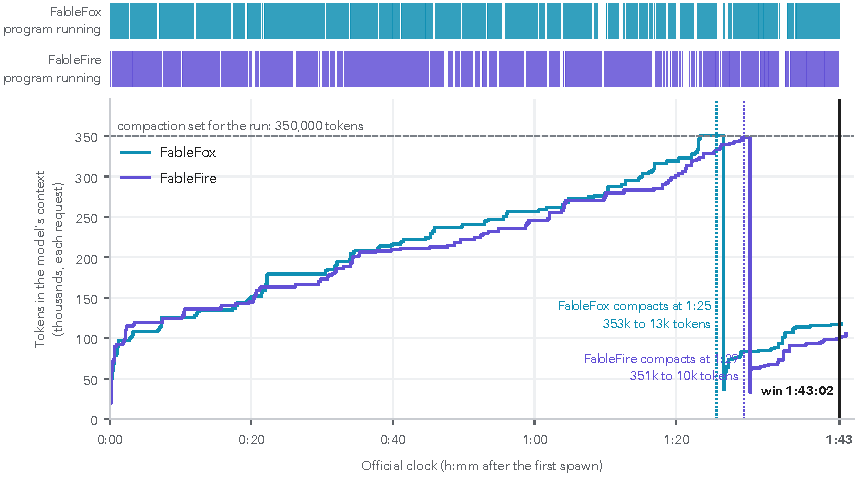
\includegraphics[width=\textwidth]{figures/fig4_context.pdf}
  \caption{Context size through the run. The lower panel shows the tokens in the model's context at each request, for each agent, with the two compactions. The upper strips show when each agent had a program running.}
  \label{fig:context}
\end{figure}

\subsection{The 5-hour and 7-day usage windows}

The subscription limits use over a rolling 5-hour window and a 7-day window, and both agents drew on the same account. Claude Code reports the share of each window used with every request (149 reports in this run). Figure~\ref{fig:usage} shows them. The 5-hour window was new when the run began: its first report read 0\%, and the rehearsal earlier in the evening had fallen in the window before. It read 82\% at the win and 84\% when the sessions ended, and was due to reset 4 hours 52 minutes after the first spawn. No request was refused. The 7-day window went from 27\% to 34\%.

Two agents filled the window at about 0.8 points a minute. At that rate it would have been full a little after the two-hour mark, with the reset almost three hours away, and paid overage is turned off on this account. An earlier two-agent experiment in this series stopped in exactly this way \citep{batsuk2026bench}. So the limit was a real constraint on this run even though it never came into play: a team of two Fable~5.2 agents on this subscription has about two hours, and this team finished with roughly twenty minutes to spare.

\begin{figure}[t]
  \centering
  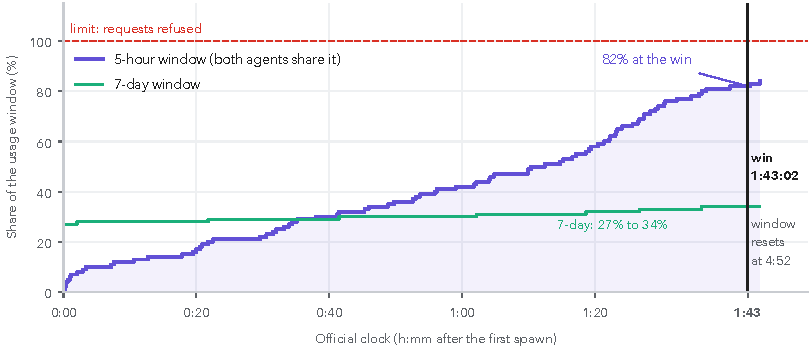
\includegraphics[width=\textwidth]{figures/fig5_usage.pdf}
  \caption{The owner's subscription usage windows through the run, from the rate-limit reports in both agents' session records. Both agents share one account, so there is one line for each window.}
  \label{fig:usage}
\end{figure}

\section{Verification and integrity}
\label{sec:verify}

The project's verification script passes for this run. The server log has one startup and the line ``Human~1 has made the advancement [Free the End]'' at the time of the harness's win event. The operator list was empty, no command was issued through the server, and the only remote-console connections were the harness's own at startup and at shutdown. No program of either agent contains a server command or a bed call outside the Overworld. The server log has no ``Can't keep up'' warnings. The camera followed FableFox and saved 618 frames up to the win, with a median gap of 10 seconds and none longer than 20. FableFire's bot connected twice, the second time after the timeout at 1:38:52; FableFox's connected once.

\section{Researcher actions}
\label{sec:researcher}

No researcher sent a message to either agent, changed a file or touched the server during play. The owner started the environment and the two sessions, and stopped the environment about four minutes after the win. The owner is not one of the players' rule-makers during a run, and Human~1 and Human~2 could talk to the agents only through the game's chat, like any player.

\section{Comparison with the earlier runs}
\label{sec:compare}

\begin{table}[t]
  \caption{This run beside the first team run and the fastest solo run. The team runs are a different experiment from the solo run; the rows are for orientation, not ranking.}
  \label{tab:compare}
  \small
  \begin{tabularx}{\textwidth}{@{}Xrrr@{}}
    \toprule
    & \textbf{This run} & \textbf{First team run} & \textbf{Run 5 (solo)} \\
    \midrule
    Agents & 2 Fable~5.2, low & 2 Opus~5.5, xhigh & 1 Fable~5.2, low \\
    People & 2 & 2 & 0 \\
    Time to \adv{Free the End} & 1:43:02 & 4:36:16 & 4:39:54 \\
    Eyes of ender & 0:53:55 & 2:52 & 1:42:05 \\
    The End entered & 1:23:18 & 3:30 & 3:32:41 \\
    Agent deaths & 1 & 7 & 4 \\
    People's deaths & 7 & 31 & -- \\
    Programs & 176 & 695 & 197 \\
    Model requests to the win & 255 & 1,111 & 246 \\
    Chat lines before the win & 198 & 367 & 0 \\
    Cost at list prices & \$36.84 & \$87.57 & \$39.52 \\
    \bottomrule
  \end{tabularx}
\end{table}

Table~\ref{tab:compare} puts the three runs side by side. Up to the Nether fortress this run was level with run 5, a few minutes ahead or behind at each step; a team gains little while every player still needs its own tools. The gap opens after the rods. Run 5's single agent spent 34 minutes getting pearls and then more than an hour and a half from the stronghold to the End, making its kit for the fight. Here the pearls were collected by a second agent and then by a person while FableFox did the rods, and the spare kits were made by FableFire while FableFox dug to the stronghold. From the first blaze rod to the open End portal took 39 minutes.

The second gap is the fight. Run 5 took 58 minutes from the last crystal to the dragon's death with a sword in a trench, and the first team run 52 minutes. This run took under eight, and the agents had almost no part in it.

Against the first team run, the largest single difference is that nothing went badly wrong. That run lost seven blaze rods and about 45 minutes to a despawn, and later half an hour to a dragon that would not perch. This one lost a kit for four minutes. With one run of each, we cannot say how much of the difference is the model, the newer plan and library, the people's practice, or luck.

\section{Related work}

\citet{faldor2026team} describe the environment and report a team of four agents defeating the dragon; our series copies their setup. Code-writing agents in Minecraft go back to Voyager \citep{wang2024voyager}, and multi-agent and human--agent play in Minecraft has been studied by \citet{white2025collaborating}, \citet{altera2024sid} and \citet{gong2024mindagent}, among others. This paper adds one more data point of a narrow kind: capable agents under fixed rules sharing a world with people who are under none.

\section{Limitations}
\label{sec:limits}

\begin{itemize}
  \item \textbf{Easy difficulty, and perception through code.} As in the earlier runs, monsters deal less damage on Easy and hunger can't kill, and Mineflayer reports exact blocks and entities to the agents.
  \item \textbf{One run.} One world, one seed, one evening. The Nether portal happened to lead near a fortress with a blaze spawner, and the stronghold was close.
  \item \textbf{The time is not a solo time, and mostly not an agents' time.} The people took about 98\% of the dragon's health after the crystals, probably by a method the agents are forbidden. A fair reading is that the agents brought the team to an open End portal by 1:20:35 and to a dragon without crystals by 1:35:28; what happened in the last eight minutes says more about the people.
  \item \textbf{Practised people.} Human~1 and Human~2 had played the first team run and a rehearsal the same evening. The agents had not, but they inherited seven earlier players' files and a plan written after the fastest of them.
  \item \textbf{The people's actions are not recorded.} The harness records the agents' programs, the chat and the server log. What the people did between chat lines, including how they fought the dragon and who broke the tenth crystal, is inferred.
  \item \textbf{The dragon's health is sampled.} It is read only when an agent's program prints it, and FableFire's readings after its reconnection were stale, so the curve uses the lowest reading so far.
  \item \textbf{The usage figures are for one subscription.} The shares of the 5-hour and 7-day windows depend on the plan and on what else the account had used that week.
  \item \textbf{No frames from the camera are shown.} The one camera followed FableFox, and its frames show the people's account names.
\end{itemize}

\section{Responsible development}

Each agent ran in a sandbox on one machine. Its shell could write only to its workspace and its team file and could connect only to its own bot's socket. It could read the other agent's workspace but not its conversation. Subagent and messaging tools were denied. Its programs could control only its own player and could neither start processes nor write files, and none of them used a server command. The people joined as survival players with no commands, under whitelisted names, through a relay limited to local-network and Tailscale addresses. Every program, model call, chat line and game event was recorded. Neither the checks above nor our reading of the logs turned up any attempt to exploit the environment or its evaluation. As far as the records show, the agents told the people the truth, reported their own failures (a death, a failed check, a short arrow count) without being asked, and gave the credit for the win to the person who made it. The people appear here only as Human~1 and Human~2, and their account names are replaced in every quote.

\section*{Data and code}

The measurements are computed from the run records by \texttt{scripts/run\_data.py}, and the figures are drawn from its output by \texttt{scripts/make\_figures.py}. Both are kept with this paper's source. The details of the narrative come from our reading of the same records. The records (programs, events, chat, server log, camera frames and transcripts) are held by the author and are not public, since they contain the people's account names. The world's seed is withheld.

\section*{Acknowledgments}

We thank Maxence Faldor, Satinder Singh and Roberta Raileanu, whose paper describes the environment we copied, and Human~1 and Human~2, who played.

Minecraft is a registered trademark of Mojang Synergies AB / Microsoft Corporation. This independent research is not approved by or affiliated with Mojang or Microsoft. The item icons in this report are from the open-source Pixel Perfection texture pack by XSSheep and Nova\_Wostra, licensed under CC BY-SA 4.0 \citep{pixelperfection}.

\bibliographystyle{abbrvnat}
\bibliography{refs}

\appendix
\section{Definitions}
\label{app:defs}

\begin{description}[leftmargin=0pt,itemsep=3pt,font=\normalfont\bfseries]
  \item[Official clock.] From the first \texttt{bot\_connected} event of either agent to the win event, taken from the server log's \adv{Free the End} line, whichever player made it: 6,182.9 seconds.
  \item[Step.] The first time any player on the team made the step's advancement, as recorded by the harness. ``Ten crystals'' is FableFire's chat line reporting that none was left.
  \item[Program.] One JavaScript program sent to a bot and recorded in an agent's programs file. A program counts as before the win if it started before the win event.
  \item[Running share.] The time covered by the union of an agent's program spans, divided by the time from its first program to the win.
  \item[Chat line.] One line of game chat as the server logged it. An agent's long message is split by the game into several lines.
  \item[Wait for an agent.] The time from a person's chat line to the next chat line by either agent (99 cases).
  \item[Model request.] One response from the model in a session's record, counted by its message identifier.
  \item[Context size.] For each request, the input tokens not cached, plus those read from the cache, plus those written to it.
  \item[Usage window.] The share of the subscription's 5-hour or 7-day allowance used, as Claude Code reported it in the session record's rate-limit events. The two sessions report one account; we plot the highest share reported so far.
  \item[Dragon's health.] The health value of the dragon entity as printed by the agents' fight programs. The curve is the running minimum of both agents' readings.
\end{description}

\end{document}
